\subsection{BPC analysis}
\subsection{BLC2-BPC matching}
\begin{figure}[htpb]
  \centering
  \begin{tabular}{cc}
    \begin{minipage}{0.5\hsize}
      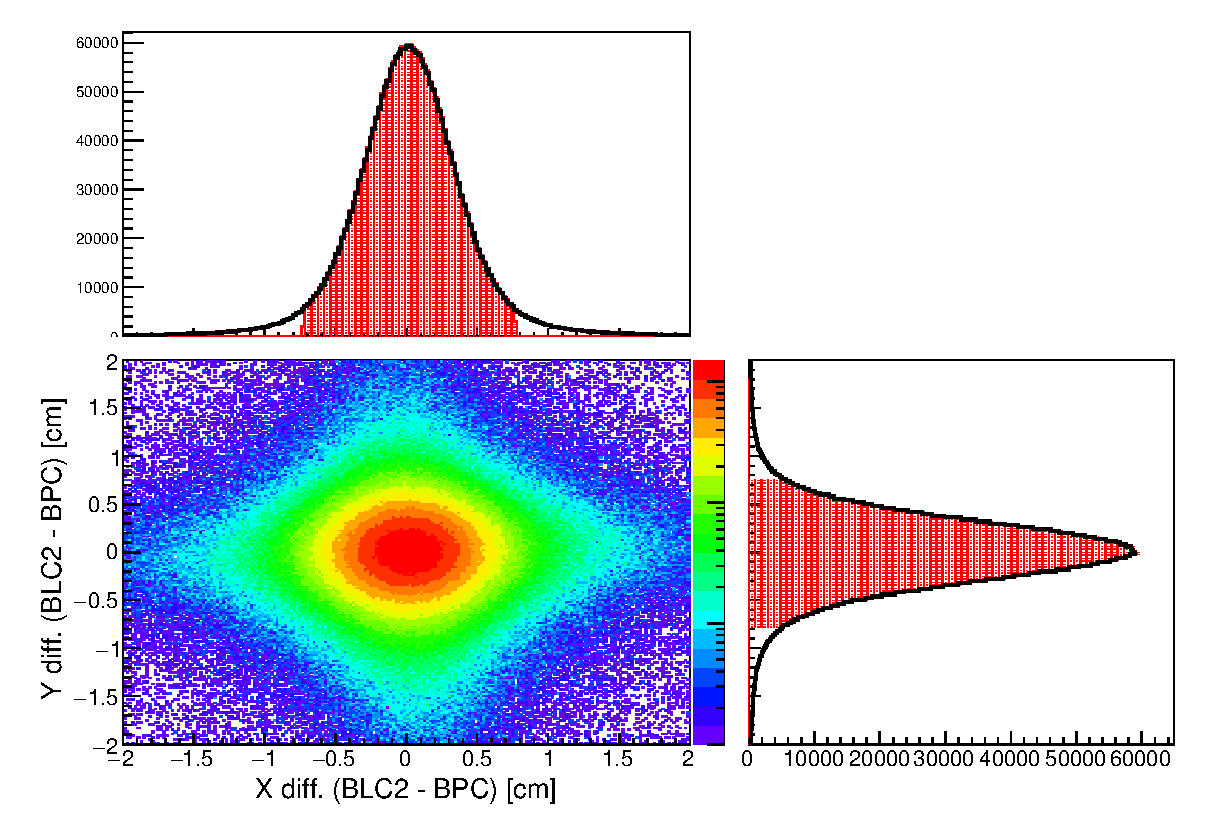
\includegraphics[width=6cm]{../pic/Run78/BL/BLC2BPC.eps}
    \end{minipage}
    \begin{minipage}{0.5\hsize}
      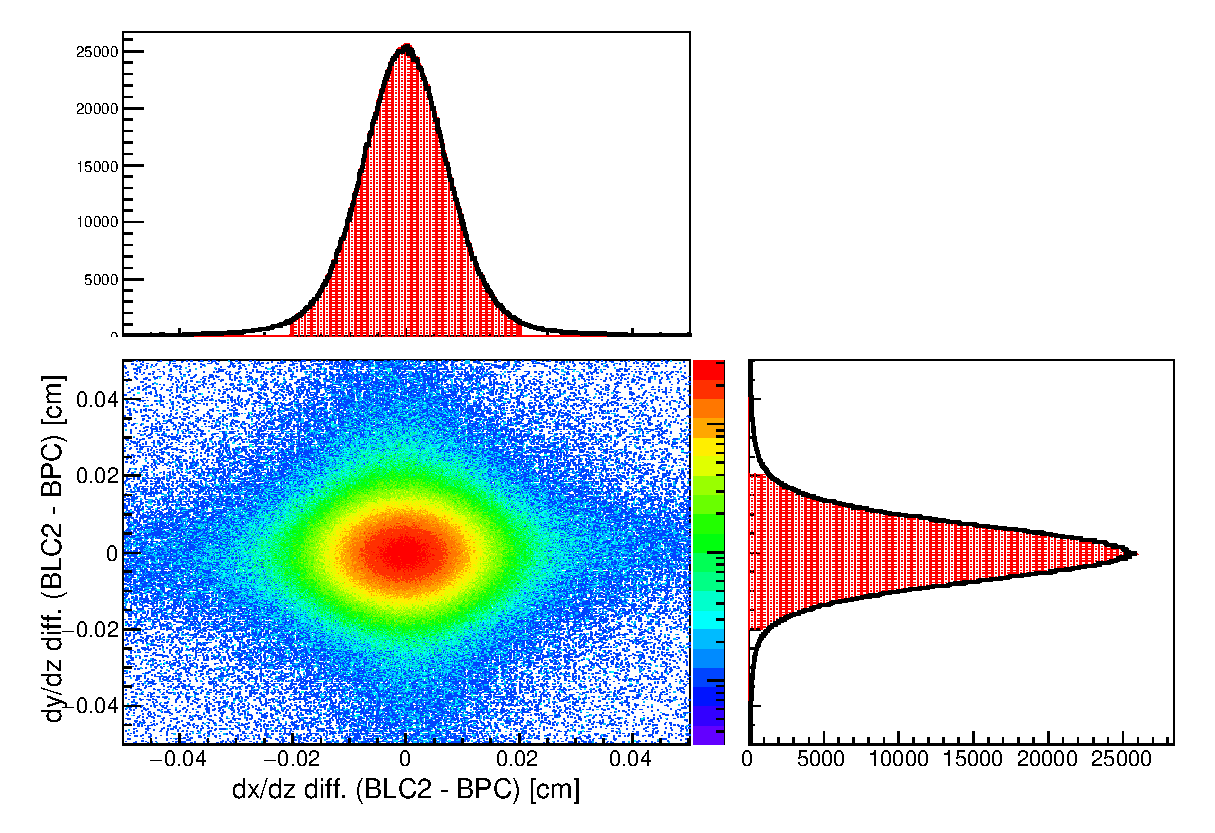
\includegraphics[width=6cm]{../pic/Run78/BL/BLC2BPC_dir.eps}
    \end{minipage}
  \end{tabular}
  \caption{
    These figures indicate the connection between the BLC2 and the BPC.
    The left figure shows about position matching at the center of these.
    The right figure shows direction matching.
    The red hatched region indicated an acceptable region.
  }
  \label{fig:BLC2BPC}
\end{figure}

\begin{figure}[htpb]
  \begin{tabular}{cc}
    \begin{minipage}{0.5\hsize}
      \includegraphics[width=6cm]{../pic/Run78/BL/profFF_Kf.eps}
    \end{minipage}
    \begin{minipage}{0.5\hsize}
      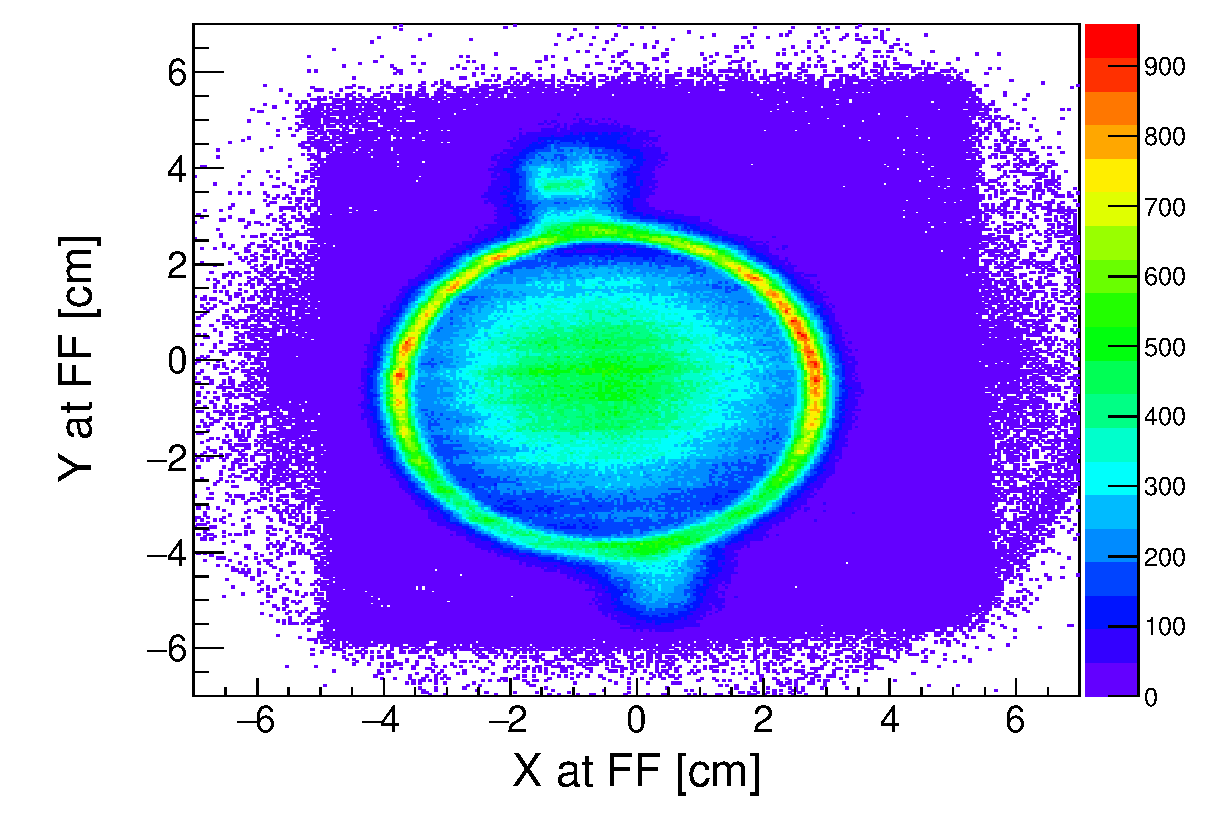
\includegraphics[width=6cm]{../pic/Run78/BL/profFF_KCDH2.eps}
    \end{minipage}
  \end{tabular}
  \caption{
    These figures shows beam profile at FF.
    The left figure shows about the unbiased kaon trigger.
    The right figure shows about CDH2 hit trigger.
  }
  \label{fig:profFF}
\end{figure}
The BPC is the same type drift chamber as BLC1/2, so the analysis of itself is the same as BLC1/2, which is shown in Fig\ref{fig:BLC_etc}.
There is no magnet between the BLC2 and the BPC, so trajectories reconstructed by them sshould be successfully connected within multiple scattering and resolution.
There are many materials between the BLC2 and the BPC, for example, the T0, the AC, BPD, and air, also direction ($dx/dz$ or $dy/dz$) resolution affects on extracted position resolution.
The $z$ length ratio of these is (BPC $z$)/(BLC2 $z$)=50.4mm/310mm$\sim$1/6, so extracted position resolution was almost decided by the BPC.
On the other hand, materials were placed at just down stream of the BLC2 for example the T0 and the AC.
These two effects were estimated almost the same, so we evaluated position matching at the center of the BLC2 and the BPC as Fig\ref{fig:BLC2BPC}.
We also require direction matching the right figure of Fig\ref{fig:BLC2BPC}.
The BPC also defines The beam profile at the experimental target position as shown in Fig\ref{fig:profFF}.
The profile required reaction at the trigger level was clearly seen target cell.
The red circle indicates an acceptable region as an effective kaon beam. %% todo Fiducialの赤枠

\begin{figure}[htpb]
  \begin{tabular}{cc}
    \begin{minipage}{0.5\hsize}
      \includegraphics[width=6cm]{../pic/Run78/BL/profFF_Kf.eps}
    \end{minipage}
    \begin{minipage}{0.5\hsize}
      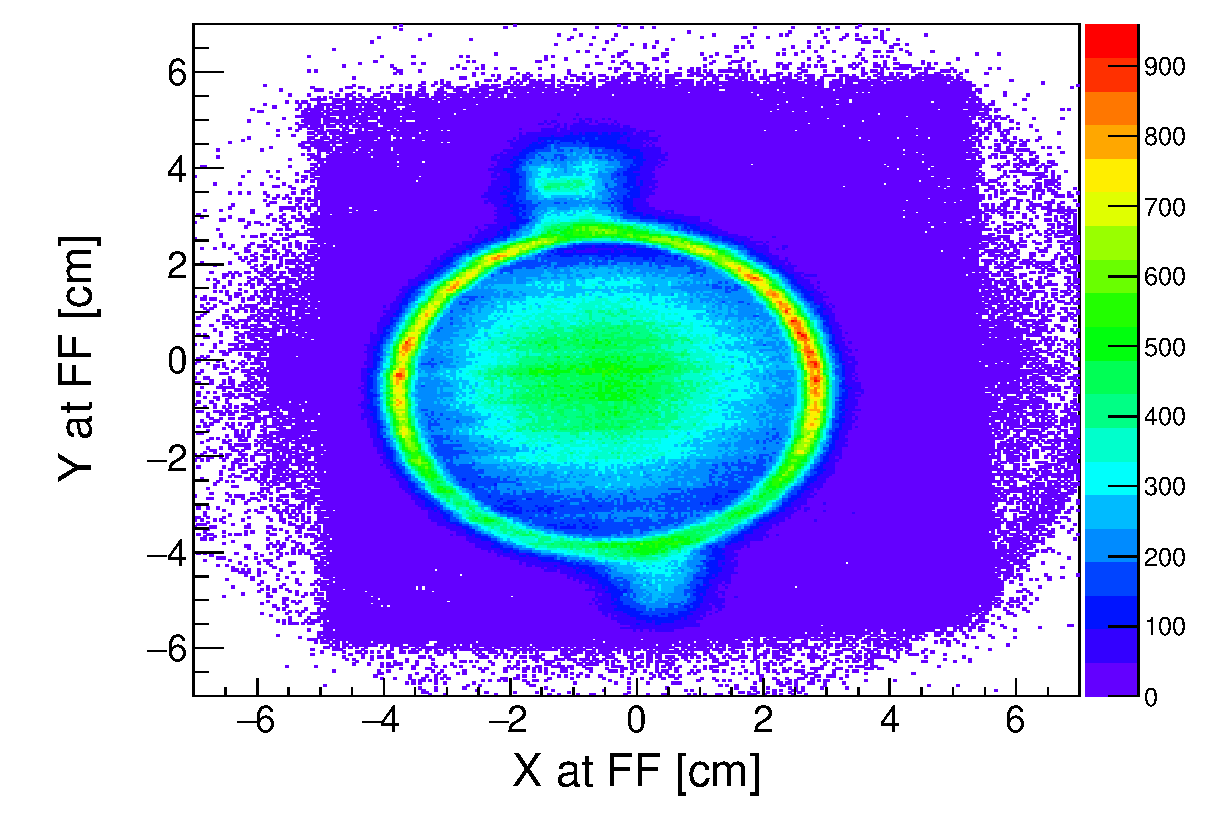
\includegraphics[width=6cm]{../pic/Run78/BL/profFF_KCDH2.eps}
    \end{minipage}
  \end{tabular}
  \caption{
    These figures shows beam profile at FF.
    The left figure shows about the unbiased kaon trigger.
    The right figure shows about CDH2 hit trigger.
  }
  \label{fig:beam_prof_fFF}
\end{figure}


The BPC 1track is selected according to the conditions of Sec.\ref{sec:BLC}.
BLC2 and BPC require those tracks to match because there is no magnet between them.
They are shown in Fig.\ref{fig:BLC2BPC}
The left figure shows the difference in position between BLC2 and BPC in the center position and the right figure shows the difference in inclination of the tracks.
A $3\sigma$ acceptance region is set for each horizontal and vertical position and inclination, all of which are accepted as the correct beam.
The acceptance regions are indicated the read hatched in thr figure.

Fig.\ref{fig:beam_prof_FF} shows the beam profile from the BPC at the centre of the liquid deuterium target.
The left figure shows one from the unbaised kaon trigger and the right figure shows one from the CDH2 trigger, which requires that the beam has reacted with the material.
Fiducial volume accepted as the Kaon beam passed through indicated the red circle.
